\documentclass[12pt]{article}
\usepackage[margin=1in]{geometry}
\usepackage{newtxtext,newtxmath}
\usepackage{amsmath,booktabs,graphicx,microtype,setspace,caption}
\usepackage{multirow,threeparttable}
\usepackage[round,semicolon]{natbib}
\usepackage[colorlinks=true,citecolor=blue,linkcolor=black,urlcolor=blue]{hyperref}
\graphicspath{{figs/}}
\captionsetup{font=small,labelfont=bf,justification=justified}
\newcommand{\gws}{\textit{GWS}}
\newcommand{\gwsp}{\ensuremath{\textit{GWS}^{\perp}}}
\onehalfspacing

\begin{document}

%---------------- Title page ----------------
\begin{titlepage}
\begin{center}
{\Large\bfseries The Cost of Silence: Conditional Under-disclosure,\\[2pt]
Price Discovery, and the Cross-Section of Stock
Returns\footnote{All code, result tables, and negative results are archived
and available from the author. All remaining errors are my own.}}\\[20pt]

{\large Wentao Liu}\\[2pt]
{\today}
\end{center}

\vspace{10pt}
\begin{center}{\bfseries Abstract}\end{center}
\begin{quote}
\singlespacing\small
\noindent
Under a voluntary ESG disclosure regime with substantial rating disagreement,
which end of the disclosure distribution does the market price? The
greenwashing literature implicitly assumes that exaggeration is punished. Using
1{,}339 Chinese A-share firms over 2014--2023, I construct a measure of
\emph{conditional under-disclosure}: the within-industry standardized gap
between a firm's ESG disclosure score and its realized ESG performance,
orthogonalized each month against six style exposures, industry fixed effects,
ESG performance, and fundamentals. What is systematically priced is not
exaggeration but \emph{silence}. The orthogonalized gap predicts one-month-ahead
returns (IC $=0.0122$, $t=3.45$, defensive timing), and the most silent decile
underperforms comparable firms by $4.17\%$ per year ($-4.16\%$, $t=-2.92$,
after the \citet{liu2019} China three-factor adjustment), with near-zero factor
loadings. Raw disclosure gaps have \emph{no} predictive power: orthogonalization
is a necessary condition for the signal to appear. Three competing explanations
are rejected. It is not greenwashing punishment---a governance-dimension
placebo is as strong as the environmental dimension, the effect is not
amplified in polluting industries, and penalty announcements generate
\emph{positive} abnormal returns ($+2.76\%$, $t=4.98$). It is not a liquidity
premium---silent firms are \emph{more} liquid, the mediation share is $7.0\%$,
and the signal survives Amihud neutralization. It is not size or quality. The
surviving channel is price discovery: the discount concentrates among stocks
with high \citet{hou2005} price delay (tail $-7.39\%$, $t=-3.54$, versus
$-3.01\%$, $t=-1.57$), and this contrast holds within the low-idiosyncratic-
volatility subsample, so it is not a restatement of limits to arbitrage.
Excluding the bottom disclosure decile from an equal-weighted portfolio earns
$0.47\%$ per year (IR $=1.07$), with incremental one-way turnover of $1.06\%$
per month and about nine-tenths of the gain surviving 30bp round-trip costs.
Results describe cross-sectional predictability rather than causal effects, the
magnitudes are modest, and the effect vanishes under value weighting.
\end{quote}

\vspace{8pt}
\noindent\textbf{JEL codes:} G12, G14, M41, Q56.\\
\textbf{Keywords:} ESG disclosure, greenwashing, price discovery, information
barriers, cross-section of returns.
\end{titlepage}

%---------------- 1 Introduction ----------------
\section{Introduction}

China's ESG market grew under a disclosure regime that was, until very
recently, almost entirely voluntary. Firms chose whether and how much to
disclose; rating agencies, in turn, leaned heavily on what firms volunteered.
The result is an information environment with two structural features: what a
firm says is partly a choice variable rather than a fact, and different
agencies reach markedly different conclusions about the same firm---in my
sample the pairwise rank correlations across three major providers range from
$0.26$ to $0.69$. In April 2024 the three Chinese exchanges issued sustainability
reporting guidelines that begin to make disclosure mandatory for index
constituents, which makes the pre-mandate period a well-defined laboratory for
a simple question: \emph{which end of the disclosure distribution does the
market price?}

The existing literature has largely studied the upper end. Work on
greenwashing \citep{yu2020,hu2023} is built on the premise that firms which
overstate their environmental credentials are eventually identified and
punished. The premise is intuitive, but the cross-sectional pricing evidence
for it in China is thin. This paper documents the opposite: \emph{what is
systematically priced is not exaggeration but silence}.

The measurement strategy is deliberately simple, and one step in it turns out
to matter more than anything else. A firm's absolute disclosure score is
contaminated by size, industry norms, and visibility, so I first standardize
disclosure and realized ESG performance within industry and take the
difference, producing a disclosure gap. I then, each month, project this gap on
six style exposures (size, book-to-market, momentum, beta, idiosyncratic
volatility, turnover), industry dummies, and ESG performance, profitability and
leverage. The residual---what I call conditional under-disclosure---answers a
narrow question: among firms that look alike in size, style, industry, and
actual ESG performance, who is relatively silent?

The first result is that this last step is not cosmetic but necessary. The raw
disclosure gap has no predictive power whatsoever (IC $=-0.0004$, $t=-0.10$).
Style neutralization alone leaves it insignificant ($0.0062$, $t=1.78$). Only
after ESG performance and fundamentals are also removed does the signal appear
(IC $=0.0136$, $t=4.23$; $0.0122$, $t=3.45$ under the most conservative timing
and standardization convention). For comparison, the ESG performance score
itself---the variable most ESG-pricing studies use---never predicts returns
once styles are removed. This asymmetry is the paper's methodological point:
disclosure behavior carries information that ESG \emph{levels} do not, but only
conditionally.

The second result characterizes where the return effect lives. Sorting on the
orthogonalized gap produces a one-sided pattern rather than a monotone one: the
most silent decile earns $0.264\%$ per month against a universe mean of
$0.612\%$, while deciles two through ten are tightly clustered. Relative to
comparable firms the silent decile loses $4.17\%$ per year ($t=-3.14$), and
$-4.16\%$ ($t=-2.92$) after adjusting for the \citet{liu2019} China three-factor
model, with essentially zero loadings on market, size, and value.

The third set of results rejects three competing explanations. \emph{It is not
greenwashing punishment.} If the market were pricing green window-dressing, the
effect should be concentrated in the environmental dimension; instead a
governance-dimension placebo is at least as strong (IC $=0.0120$, $t=3.62$,
versus $0.0099$, $t=3.37$) even though the two component factors correlate only
$0.18$. The effect is not amplified in heavily polluting industries. And in an
event study around 2{,}094 hand-collected penalty announcements, high-gap firms
earn \emph{positive} cumulative abnormal returns of $+2.76\%$ ($t=4.98$)---the
opposite sign to what "exposure of greenwashing" predicts, and consistent with
Chinese penalty filings typically being published jointly with confirmation of
remediation, so that the filing resolves uncertainty rather than creating it.
\emph{It is not a liquidity premium.} Silent firms are, if anything,
\emph{more} liquid conditional on size and turnover; the liquidity channel
mediates only $7.0\%$ of the total effect; and adding log-Amihud illiquidity to
the neutralization leaves predictive power essentially intact ($0.0136 \to
0.0128$, $t=3.90$). \emph{It is not size or quality}: the effect is stronger in
the large-cap half, and the signal is orthogonal to a standard quality
composite (correlation $0.001$) while retaining a Fama-MacBeth marginal
$t$ of $3.68$ on top of it.

The fourth result identifies the channel that survives. Using
\citet{hou2005} price delay, the silence discount concentrates precisely where
prices absorb market information slowly: in the high-delay half the most silent
decile loses $7.39\%$ per year ($t=-3.54$) versus $3.01\%$ ($t=-1.57$) in the
low-delay half. Because delay correlates with idiosyncratic volatility
($\rho=0.37$), and high idiosyncratic volatility is the standard proxy for
limits to arbitrage, I repeat the split inside the low-volatility subsample;
delay still separates the two groups ($-5.94\%$, $t=-3.11$, versus $-3.43\%$,
$t=-1.93$). Price-discovery speed therefore carries information beyond
arbitrage frictions. Together with the event study, the picture is a barrier
that is raised, priced while it stands, and repriced when it is removed.

Finally, the economic magnitudes are real but small, and I report them as such.
Excluding the bottom disclosure decile from an equal-weighted portfolio
generates $0.47\%$ per year with a tracking error of $0.45\%$ (IR $=1.07$).
Because the exclusion list covers only a tenth of the portfolio, incremental
one-way turnover is $1.06\%$ per month and roughly nine-tenths of the gain
survives 30bp round-trip costs. Under value weighting the excess return
disappears, so the economic relevance is confined to equal-weighted or
small-cap-tilted implementations.

\medskip
\noindent\textbf{What this paper does and does not claim.} This is a study of
cross-sectional \emph{predictability}, not of causal effects. Disclosure is a
choice, and the neutralization controls observables only. I attempted to use
the April 2024 disclosure mandate as a quasi-natural experiment and report in
Section~\ref{sec:robust} why that test cannot identify anything in the current
data: the mandate was announced the same day as a major market-structure policy
that triggered a large-cap/small-cap divergence, my treatment proxy is
constructed from market capitalization and thus overlaps that shock, and the
event window coincides with a period in which the baseline effect had itself
reversed. I keep the negative result rather than discarding it.

\medskip
\noindent\textbf{Related literature.} This paper connects three strands. The
first is the greenwashing literature \citep{yu2020,hu2023}, whose maintained
hypothesis---that overstatement is punished---I test directly and reject in the
Chinese cross-section, while confirming \citet{hu2023}'s "green fog"
intuition in a different form: the tail discount is deepest where rating
agencies disagree most. The second is the asset-pricing literature on
incomplete information: \citet{merton1987} on investor recognition and
\citet{easley2004} on information risk both imply that information barriers
should be priced, though neither pins down whether the consequence is
compensation for risk or slow-moving mispricing; my evidence favors the
latter. The third is the price-discovery literature, in particular
\citet{hou2005}, whose delay measure provides the channel test that
discriminates between the two mechanisms considered here.

%---------------- 2 Setting and hypotheses ----------------
\section{Institutional setting and hypotheses}

\subsection{Setting}
Before the April 2024 guidelines, ESG reporting by Chinese listed firms was
voluntary apart from narrow sector rules; by the end of 2024 roughly 2{,}200
listed firms published an ESG or CSR report, with wide variation in quality and
comparability. Two consequences matter here. First, disclosure quantity is
itself an input to ratings, so "discloses a lot" and "performs well" are hard
to separate within any single rating. Second, agencies disagree: the pairwise
rank correlations among the three providers used in Section~\ref{sec:hetero}
are $0.685$, $0.453$, and $0.255$.

\subsection{Hypotheses}
\citet{merton1987} shows that securities investors do not know about require
higher expected returns; \citet{easley2004} shows that securities with greater
information asymmetry command higher required returns. Both imply that
information barriers are priced, but the direction of the return effect depends
on whether the barrier operates as compensated risk or as slow-moving
mispricing. This motivates:

\begin{quote}
\noindent\textbf{H1 (silence discount).} Conditional on size, style, industry,
and realized ESG performance, relatively under-disclosing firms earn lower
future returns.

\noindent\textbf{H2 (liquidity channel).} Under-disclosing firms are less
liquid, and liquidity differences account for a substantial part of the
discount.

\noindent\textbf{H3 (price-discovery channel).} Under-disclosing firms exhibit
higher price delay, and the discount is concentrated among firms whose prices
adjust slowly.

\noindent\textbf{H4 (barrier removal).} When information is released by
regulatory compulsion, firms with previously higher barriers experience a
significant price reaction.
\end{quote}

\noindent The greenwashing literature's implicit hypothesis---that \emph{high}
disclosure gaps predict low returns---is the mirror image of H1 and is treated
throughout as the competing hypothesis.

%---------------- 3 Data and measurement ----------------
\section{Data and measurement}

\subsection{Sample}
ESG disclosure scores are Bloomberg ESG disclosure scores (0--100, measuring
breadth and granularity of disclosure); ESG performance is the numerical rating
of a major domestic Chinese ESG rating provider.\footnote{The exact provider
should be confirmed against the data manual before submission; the empirical
design requires only that the performance leg be a rating not mechanically
driven by disclosure quantity.} Accounting data are from CSMAR. After merging
and cleaning, the annual panel covers 2014--2023 with 9{,}835 firm-year
observations on 1{,}339 firms in 71 industries. Daily prices for the entire
A-share market (January 2014 to December 2024) are used to build monthly
returns, style factors, and the liquidity and price-discovery measures.
Merging the annual signal with monthly returns yields 120 monthly cross-sections
from January 2015 to December 2024 (119 with forward returns), 116{,}244
stock-months, and 969 stocks per month on average.

\subsection{Conditional under-disclosure}
The disclosure gap is
\begin{equation}
\gws_{i,t} = z\!\left(\textit{Disclosure}_{i,t}\mid \textit{Ind}_i\right)
           - z\!\left(\textit{Performance}_{i,t}\mid \textit{Ind}_i\right),
\end{equation}
where $z(\cdot\mid \textit{Ind})$ denotes within-industry cross-sectional
standardization. Low values identify firms that do relatively more than they
say. Each month I then estimate
\begin{equation}
\gws_{i,t} = \alpha_t + \sum_k \beta_{k,t}\,\textit{Style}_{k,i,t}
           + \sum_j \gamma_{j,t}\,\textit{Ind}_{j,i}
           + \delta_t'\,\textit{Fund}_{i,t} + \varepsilon_{i,t},
\end{equation}
where \textit{Style} contains log market capitalization, book-to-market,
momentum (cumulative return from $t-12$ to $t-2$), beta (250 trading days
against the CSI All-Share index), idiosyncratic volatility, and turnover, each
standardized and winsorized at $\pm 3$; \textit{Fund} contains the ESG
performance score, ROA, and leverage. The residual \gwsp{} is the paper's
explanatory variable.

\subsection{Timing}
Year-$t$ ESG scores carry an accounting period ending 31 December of year $t$,
so they are computed from annual reports that are published between April and
June of $t+1$. I therefore report two conventions. Under \emph{baseline timing}
the year-$t$ signal is applied to the twelve monthly cross-sections of calendar
year $t+1$. Under \emph{defensive timing}---the paper's primary
specification---it is applied from July of $t+1$ for the following twelve
months, and industry standardization is replaced by industry-by-year
standardization so that no standardization constant is reused across years.
Tables report both.

%---------------- 4 Main results ----------------
\section{The silence discount}

\subsection{Orthogonalization is necessary}
Table~\ref{tab:ic} and Figure~\ref{fig:levels} report predictive power at three
levels of processing. The raw gap predicts nothing; style neutralization alone
is insufficient; only after ESG performance and fundamentals are removed does
the signal emerge. The ESG performance score itself, by contrast, never
survives style neutralization. This is the central measurement result: what is
informative is disclosure \emph{conditional} on everything that ordinarily
drives it.

\begin{table}[t]
\centering\small
\caption{\textbf{Cross-sectional predictive power by level of processing.} IC
is the Pearson correlation between the signal and the next month's return
computed within each monthly cross-section; RankIC is its Spearman analogue.
ICIR is the mean IC divided by its standard deviation across months, and $t$
multiplies the ICIR by $\sqrt{T}$. Baseline timing uses $T=119$ months
(2015:01--2024:12); defensive timing uses $T=113$.}
\label{tab:ic}
\vspace{6pt}
\begin{tabular}{lcccccc}
\toprule
Signal & IC & ICIR & $t$(IC) & RankIC & $t$(RankIC) & \% pos. \\
\midrule
\gws{} raw                       & $-0.0004$ & $-0.01$ & $-0.10$ & $-0.0052$ & $-1.08$ & 48.7 \\
\quad + style                    & $+0.0062$ & $0.16$ & $1.78$ & $+0.0037$ & $1.06$ & 54.6 \\
\quad + style + ESG/fundamentals & $\mathbf{+0.0136}$ & $\mathbf{0.39}$ & $\mathbf{4.23}$ & $\mathbf{+0.0124}$ & $\mathbf{3.45}$ & 64.7 \\
\midrule
ESG performance raw              & $+0.0034$ & $0.04$ & $0.48$ & $+0.0096$ & $1.26$ & 46.2 \\
\quad + style                    & $+0.0046$ & $0.11$ & $1.21$ & $+0.0052$ & $1.48$ & 56.3 \\
\midrule
Defensive timing (primary)       & $+0.0122$ & $0.32$ & $3.45$ & $+0.0103$ & $2.87$ & 62.8 \\
\bottomrule
\end{tabular}
\end{table}

\begin{figure}[t]
\centering
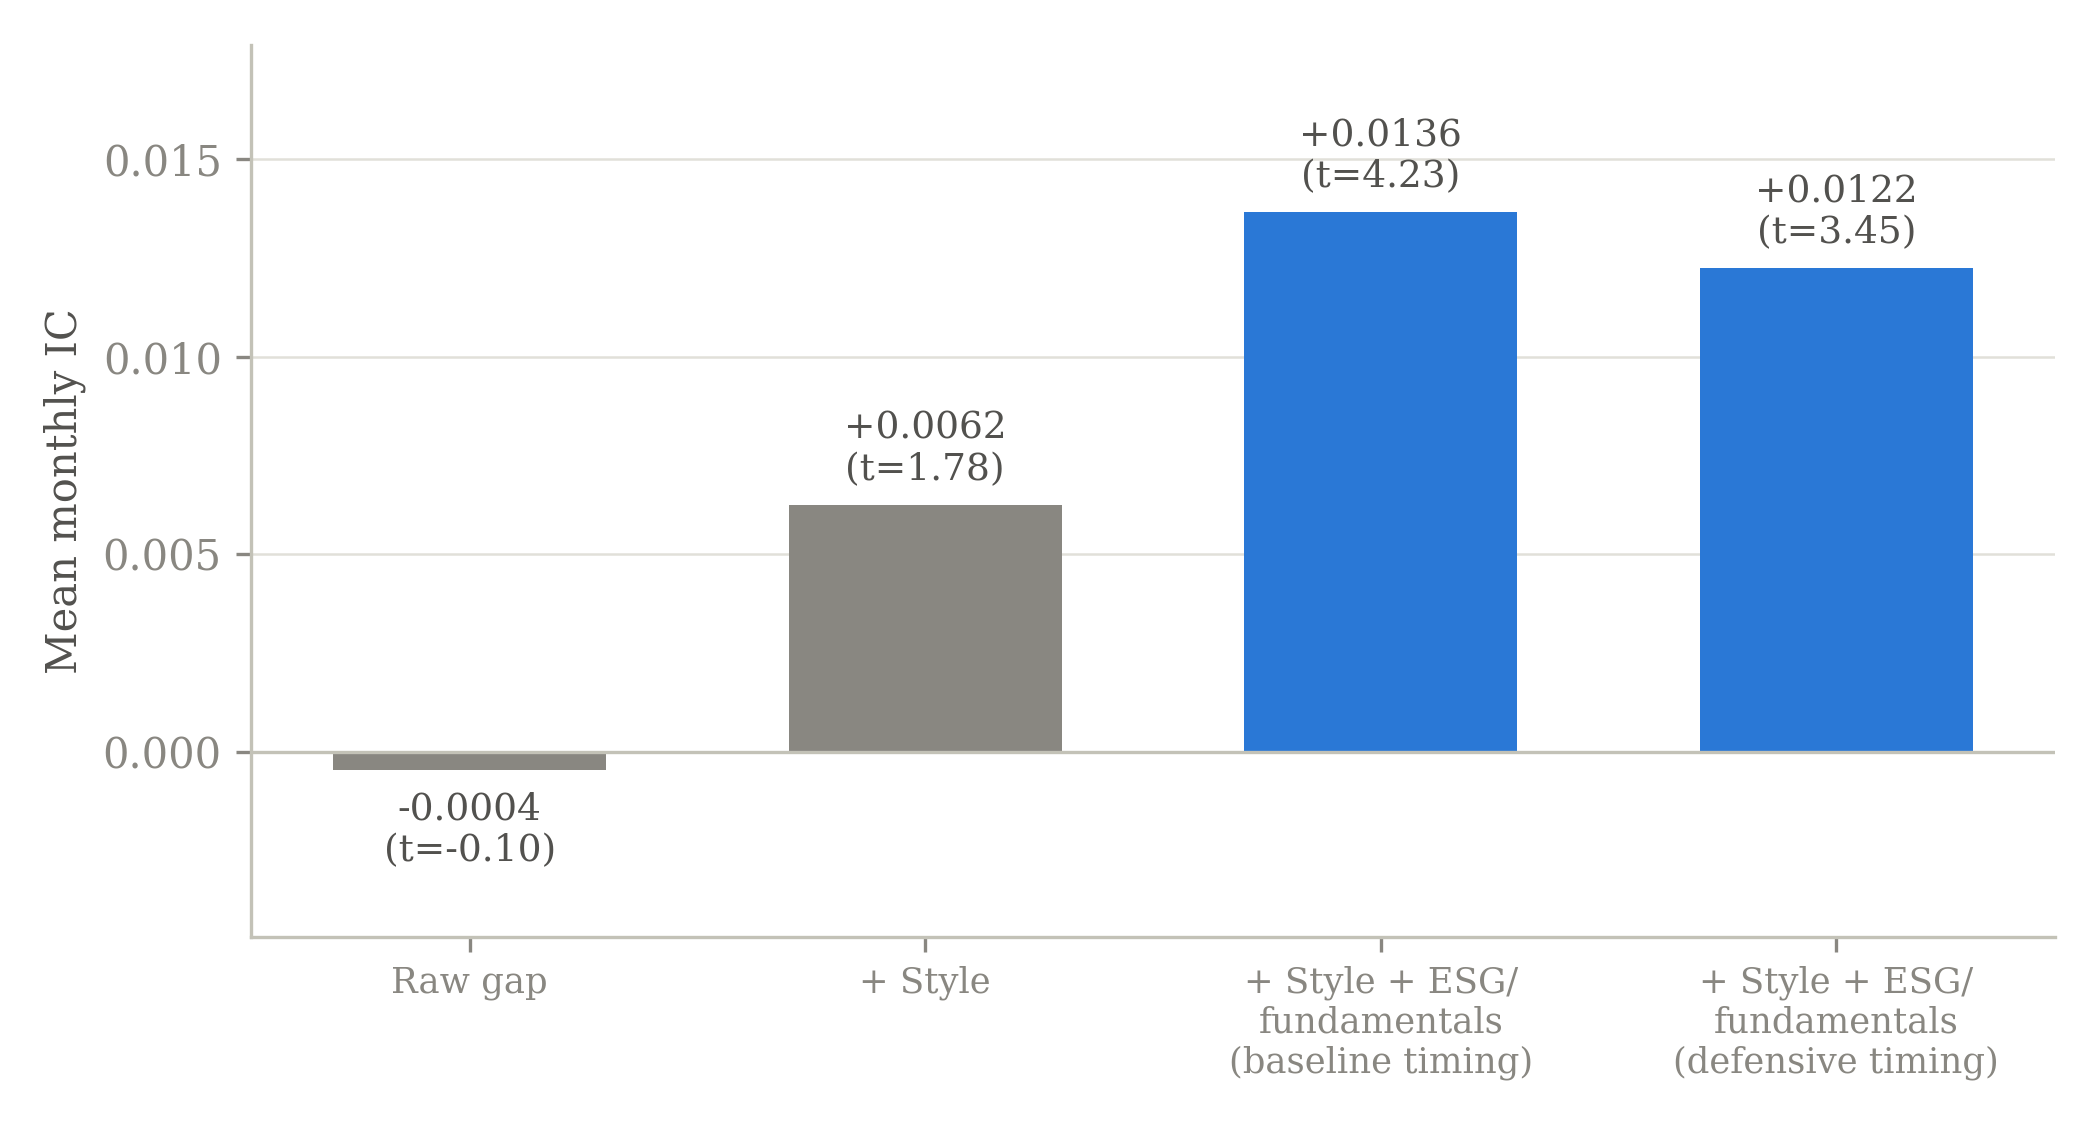
\includegraphics[width=0.82\textwidth]{fig1.png}
\caption{\textbf{Orthogonalization steps and predictive power.} Bars are mean
monthly ICs with $t$-statistics in parentheses. Grey bars denote incompletely
neutralized specifications.}
\label{fig:levels}
\end{figure}

\subsection{Portfolio sorts}
Table~\ref{tab:decile} and Figure~\ref{fig:decile} show that the effect is
one-sided. The most silent decile earns $0.264\%$ per month against a universe
mean of $0.612\%$; deciles two through ten differ little from one another. The
long-short portfolio earns $4.44\%$ per year with a Sharpe ratio of $0.79$
($t=2.42$), and the silent decile loses $4.17\%$ per year relative to
comparable firms ($t=-3.14$). Figure~\ref{fig:nav} plots cumulative values and
Figure~\ref{fig:ic} the monthly RankIC series. The one-sidedness has a direct
implication for implementation, developed in Section~\ref{sec:econ}: the signal
should be used as an exclusion flag rather than as a linear score.

\begin{table}[t]
\centering\small
\caption{\textbf{Average next-month returns by conditional under-disclosure
decile.} Defensive timing. D1 contains the most silent firms. The long-short
portfolio (D10 $-$ D1) earns $4.44\%$ per year with a Sharpe ratio of $0.79$
($t=2.42$) and a maximum drawdown of $-10.25\%$.}
\label{tab:decile}
\vspace{6pt}
\begin{tabular}{lccccccccccc}
\toprule
& D1 & D2 & D3 & D4 & D5 & D6 & D7 & D8 & D9 & D10 & Universe \\
\midrule
Return (\%) & $\mathbf{0.264}$ & 0.407 & 0.606 & 0.637 & 0.651 & 0.661 & 0.627 & 0.788 & 0.847 & 0.634 & 0.612 \\
\bottomrule
\end{tabular}
\end{table}

\begin{figure}[t]
\centering
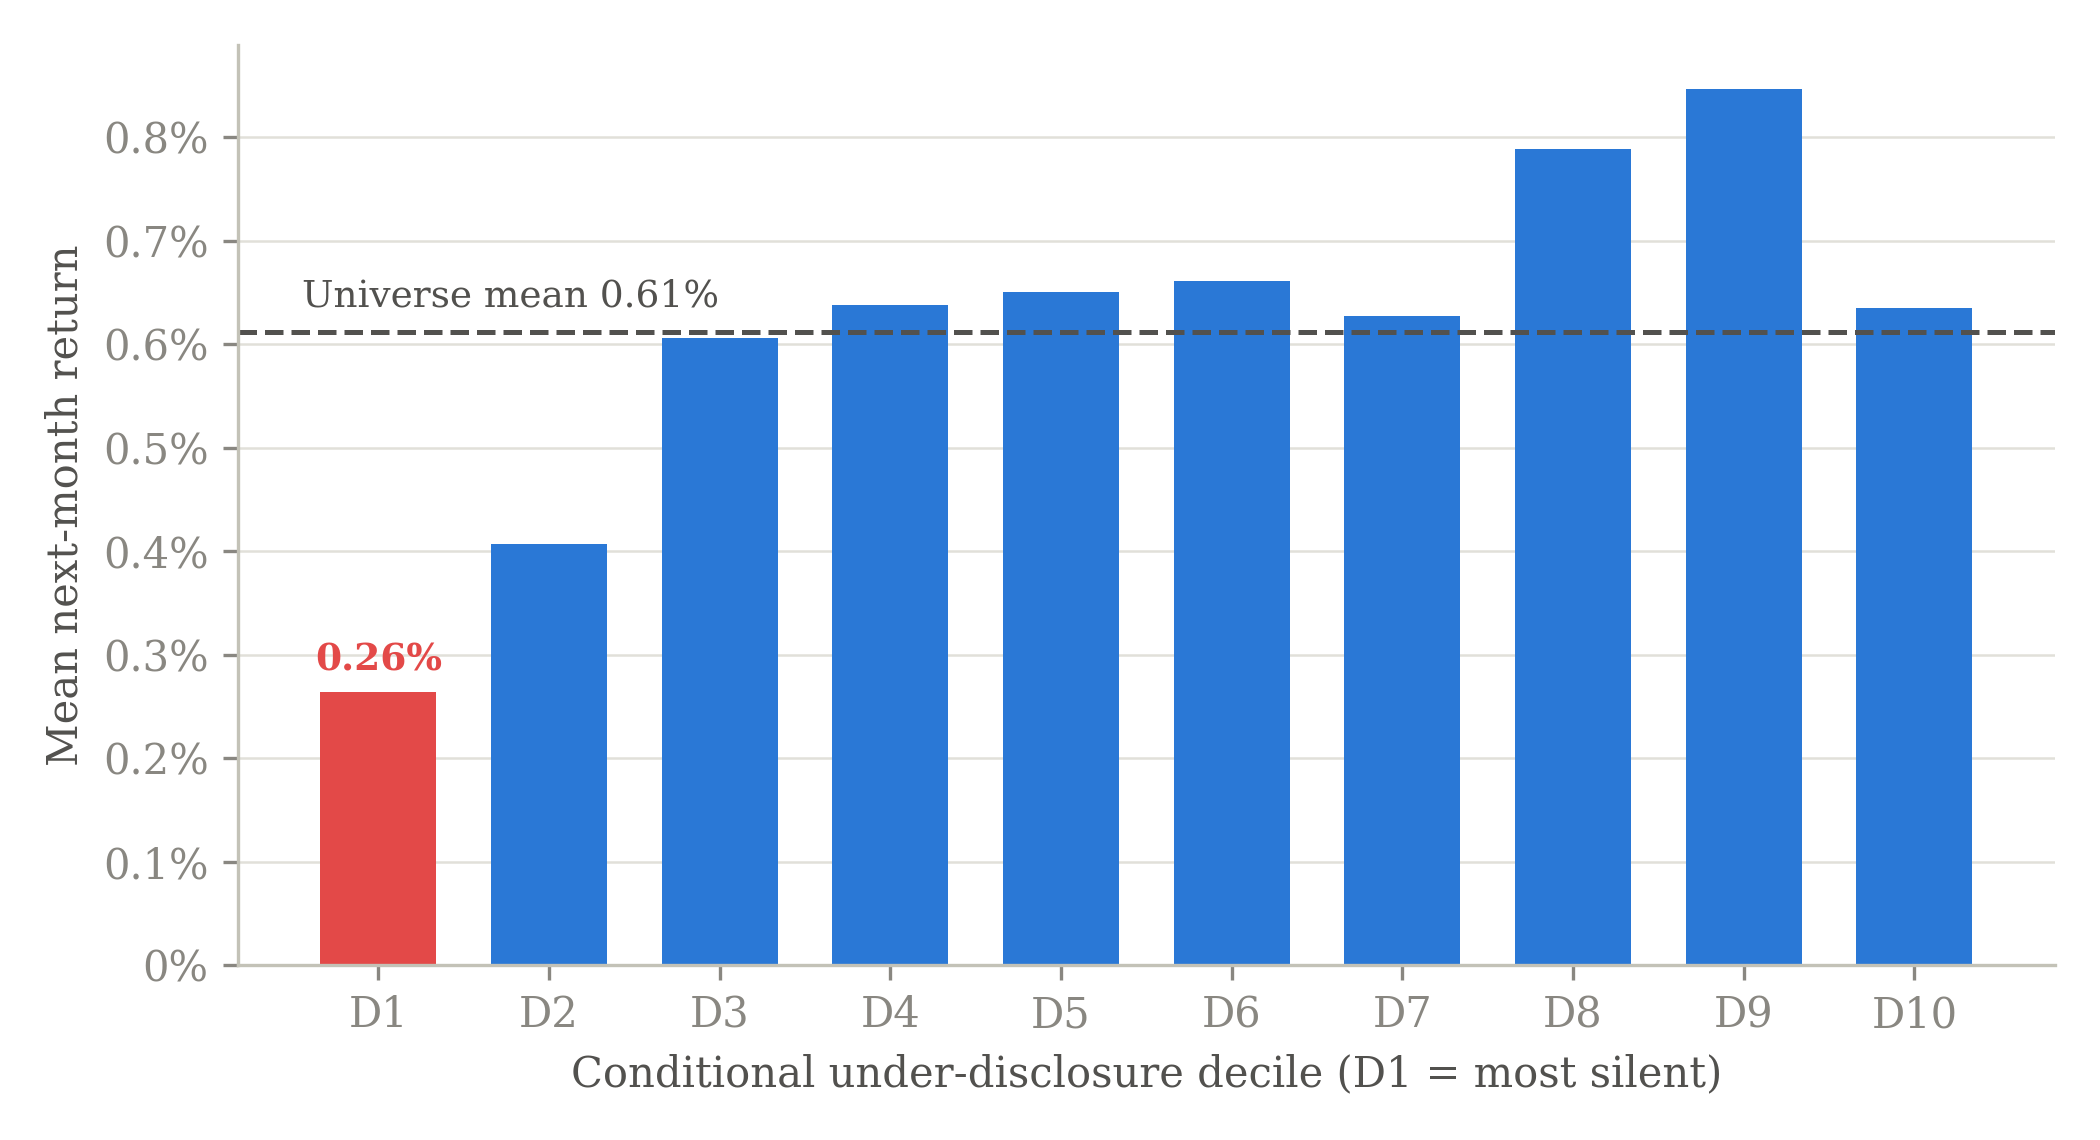
\includegraphics[width=0.82\textwidth]{fig2.png}
\caption{\textbf{Average next-month returns by decile} (defensive timing).}
\label{fig:decile}
\end{figure}

\begin{figure}[t]
\centering
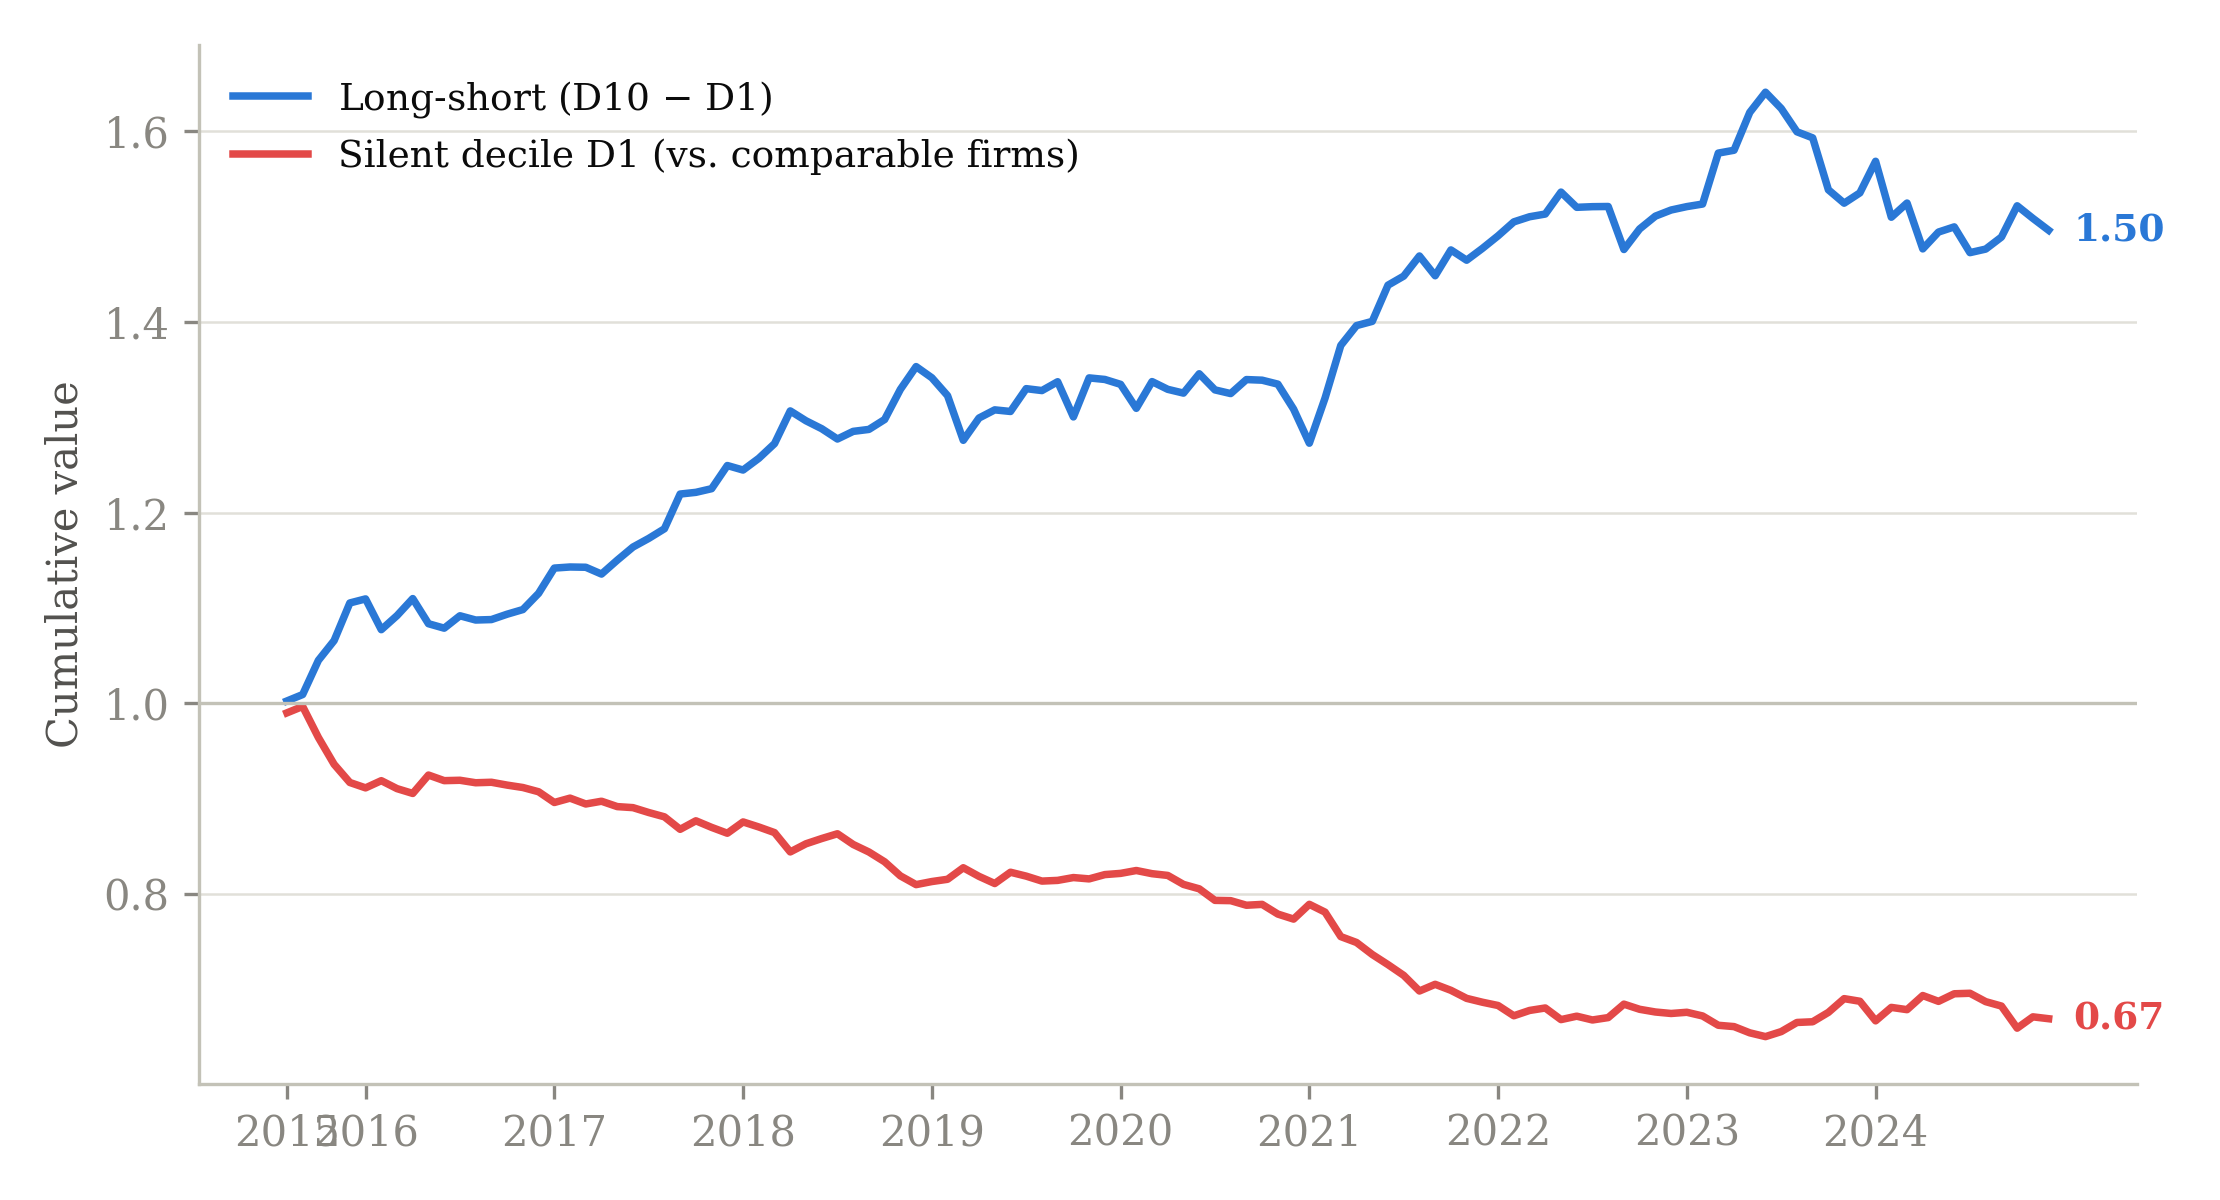
\includegraphics[width=0.86\textwidth]{fig3.png}
\caption{\textbf{Cumulative value of the long-short portfolio and of the silent
decile relative to comparable firms} (defensive timing).}
\label{fig:nav}
\end{figure}

\begin{figure}[t]
\centering
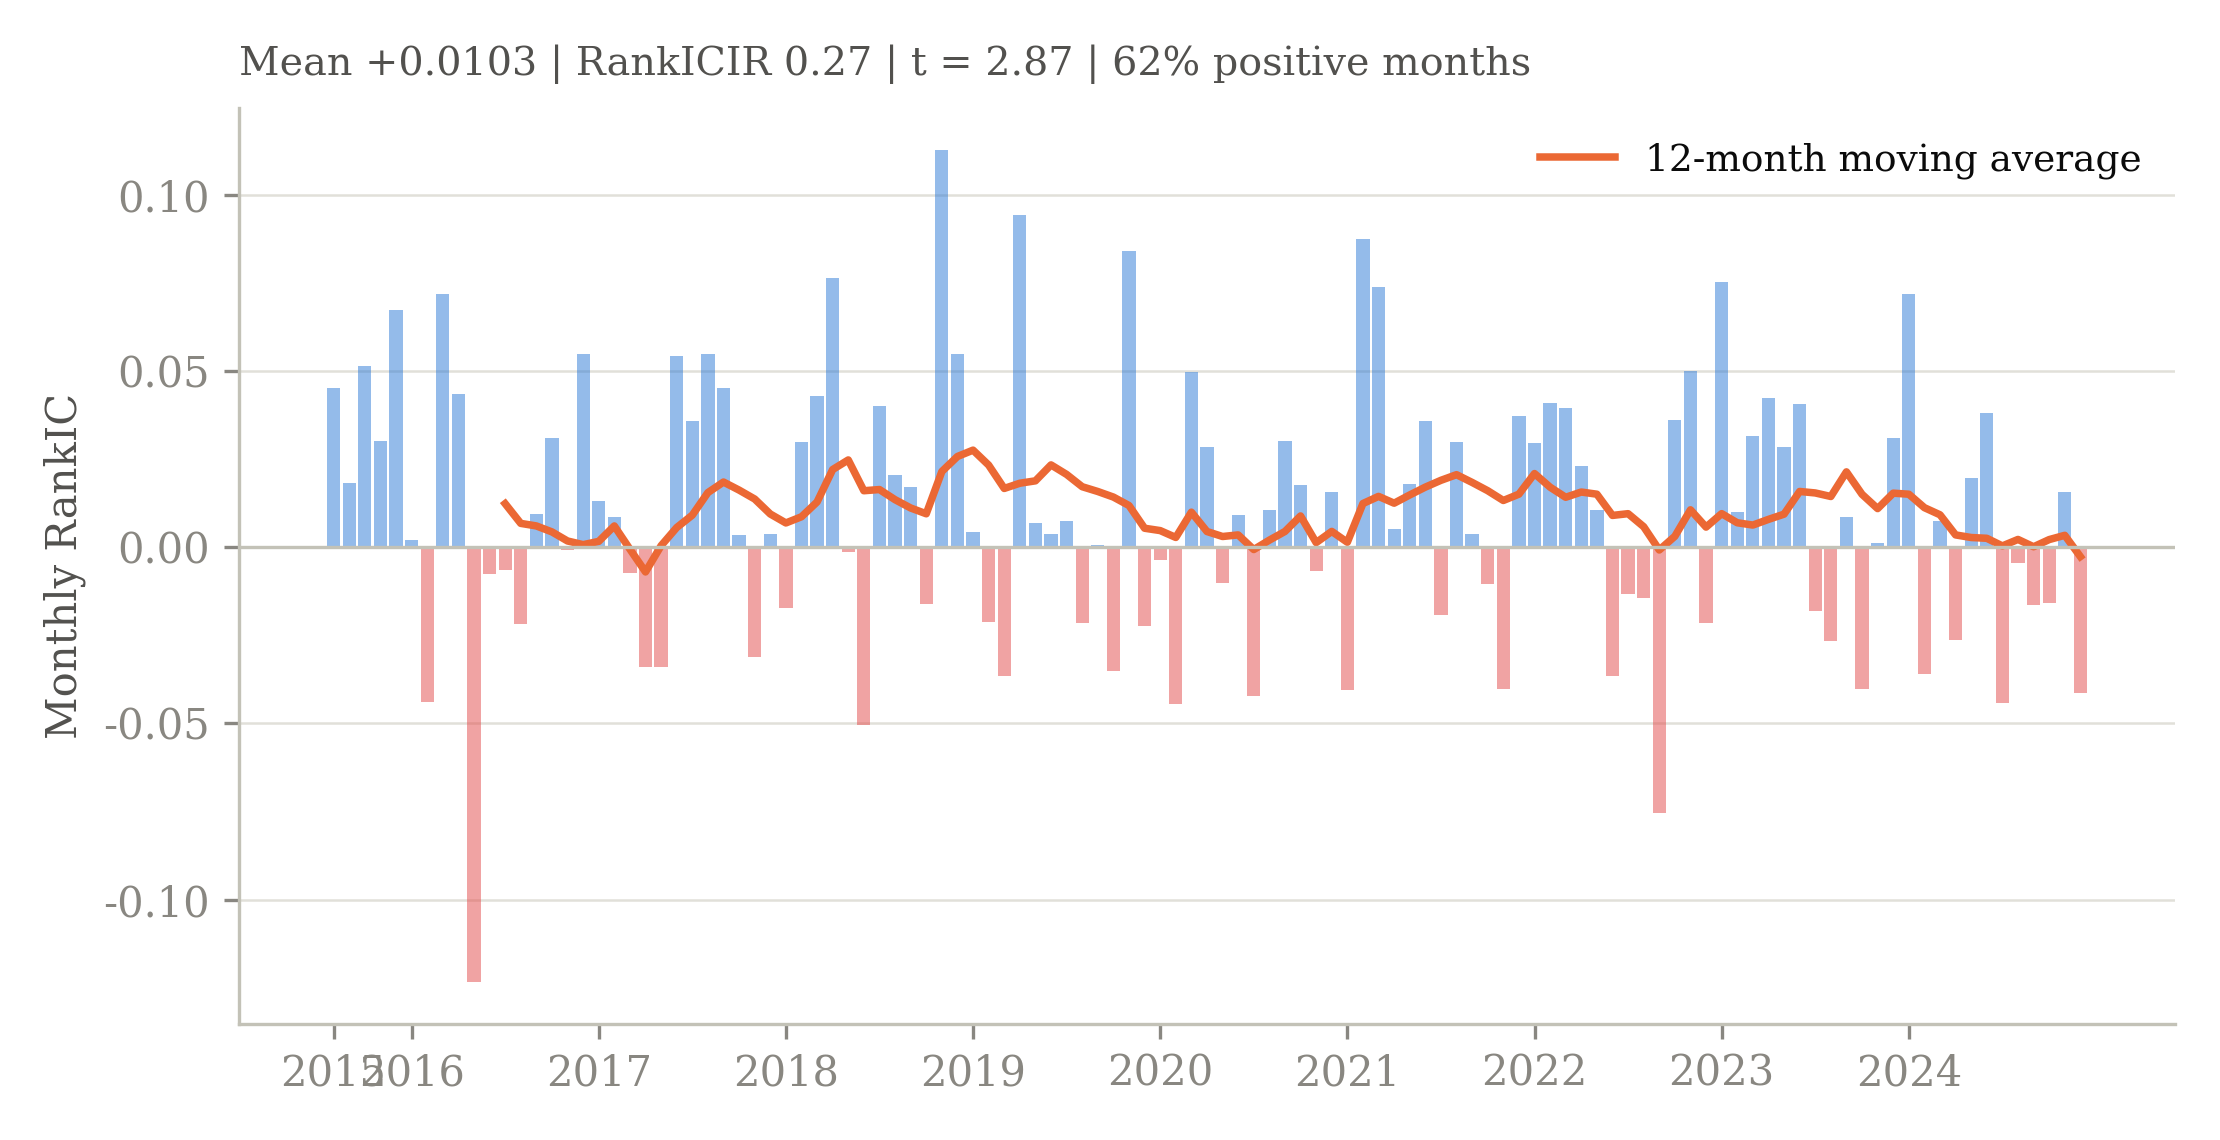
\includegraphics[width=0.86\textwidth]{fig4.png}
\caption{\textbf{Monthly RankIC and its twelve-month moving average}
(defensive timing).}
\label{fig:ic}
\end{figure}

\subsection{Risk-adjusted alphas}
Table~\ref{tab:alpha} regresses portfolio returns on the CAPM, on
Fama-French three factors, and on the China three factors of \citet{liu2019},
which I construct from the same daily data: the smallest $30\%$ of firms by
market capitalization are dropped to avoid shell-value contamination, value is
measured by earnings-to-price, and the six $2\times 3$ portfolios are value
weighted. Over the sample the market, size, and value factors earn $7.14\%$,
$3.19\%$, and $9.53\%$ per year. Standard errors follow \citet{newey1987} with
six lags.

Two features deserve emphasis. First, the silent-decile discount and the
exclusion portfolio's gain are significant at the $1\%$ level under every
model, whereas the long-short alpha under the most conservative combination
(defensive timing, Fama-French three factors) reaches only $t=1.78$---a pattern
consistent with the information residing in the lower tail. Second, the
"silent decile" rows measure performance \emph{relative to the equal-weighted
coverage universe}. In absolute terms the silent decile's China three-factor
alpha is only $-0.25\%$ ($t=-0.18$) while the top decile earns $3.62\%$
($t=2.21$), because the coverage universe---Bloomberg-covered and therefore
large-cap tilted---itself carries a positive alpha against the three-factor
model. The correct statement is that silent firms are discounted relative to
comparable firms, not that they lose money in absolute terms.

\begin{table}[t]
\centering\small
\caption{\textbf{Risk-adjusted alphas.} Annualized intercepts from time-series
regressions of monthly portfolio returns on the CAPM, the Fama-French three
factors, and the \citet{liu2019} China three factors (CH-3). The main panel
uses defensive timing ($T=113$); the bottom panel repeats the exercise under
baseline timing ($T=119$). Standard errors are \citet{newey1987} with six lags.
Portfolios in the first three blocks are hedged or relative and are not
adjusted for the risk-free rate.}
\label{tab:alpha}
\vspace{6pt}
\begin{tabular}{llccccc}
\toprule
Portfolio & Model & $\alpha$ (ann.) & $t$ & $\beta_{MKT}$ & $\beta_{SMB}$ & $\beta_{VAL}$ \\
\midrule
\multirow{3}{*}{Silent decile D1 (vs.\ universe)}
 & CAPM & $-4.17\%$ & $-3.04$ & $0.00$ & & \\
 & CH-3 & $\mathbf{-4.16\%}$ & $\mathbf{-2.92}$ & $0.02$ & $-0.11$ & $0.00$ \\
 & FF3  & $-3.42\%$ & $-2.65$ & $0.01$ & $-0.10$ & $-0.02$ \\
\midrule
\multirow{3}{*}{Exclusion portfolio (drop bottom 10\%)}
 & CAPM & $+0.47\%$ & $3.03$ & $0.00$ & & \\
 & CH-3 & $\mathbf{+0.46\%}$ & $\mathbf{2.91}$ & $0.00$ & $0.01$ & $0.00$ \\
 & FF3  & $+0.38\%$ & $2.65$ & $0.00$ & $0.01$ & $0.00$ \\
\midrule
\multirow{3}{*}{Long-short (D10 $-$ D1)}
 & CAPM & $+4.49\%$ & $2.59$ & $-0.03$ & & \\
 & CH-3 & $+3.88\%$ & $2.08$ & $-0.03$ & $0.15$ & $0.05$ \\
 & FF3  & $+3.27\%$ & $1.78$ & $-0.03$ & $0.13$ & $0.06$ \\
\midrule
\multicolumn{7}{l}{\emph{Baseline timing (comparison)}} \\
Silent decile D1        & CH-3 & $-4.63\%$ & $-4.00$ & $0.01$ & $-0.17$ & $-0.01$ \\
Exclusion portfolio     & CH-3 & $+0.52\%$ & $4.00$ & $0.00$ & $0.02$ & $0.00$ \\
Long-short              & CH-3 & $+5.30\%$ & $3.38$ & $-0.01$ & $0.07$ & $0.04$ \\
\bottomrule
\end{tabular}
\end{table}

%---------------- 5 What it is not ----------------
\section{What the effect is not}

\subsection{Not greenwashing punishment: a governance placebo}
If the market priced green window-dressing, the effect should be specific to
the environmental dimension. Table~\ref{tab:esg} constructs separate gaps from
Bloomberg's E, S, and G disclosure sub-scores. The governance gap is at least
as predictive as the environmental gap even though the two component factors
correlate only $0.183$; an equal-weighted composite of the three adds nothing
over the aggregate gap (IC $=0.0132$, $t=4.18$). Two nearly orthogonal signals
with equal predictive power indicate a common component---disclosure behavior
across dimensions---rather than anything specific to environmental claims.

\begin{table}[t]
\centering\small
\caption{\textbf{E/S/G sub-dimension gaps: a placebo test.} Each row
constructs the gap using the corresponding Bloomberg disclosure sub-score in
place of the aggregate. Pairwise correlations of the resulting factors are
$0.183$ (E,G), $0.475$ (E,S), and $0.120$ (S,G). Baseline timing, $T=119$.}
\label{tab:esg}
\vspace{6pt}
\begin{tabular}{lcccc}
\toprule
Signal & IC & $t$(IC) & RankIC & $t$(RankIC) \\
\midrule
Aggregate gap & $+0.0136$ & $4.23$ & $+0.0124$ & $3.45$ \\
Environmental (E) gap & $+0.0099$ & $3.37$ & $+0.0067$ & $1.90$ \\
Social (S) gap & $+0.0066$ & $2.27$ & $+0.0050$ & $1.55$ \\
Governance (G) gap \emph{(placebo)} & $\mathbf{+0.0120}$ & $\mathbf{3.62}$ & $\mathbf{+0.0094}$ & $\mathbf{2.75}$ \\
\bottomrule
\end{tabular}
\end{table}

\subsection{Not greenwashing punishment: polluting industries}
Incentives to greenwash are strongest in heavily polluting industries. Using
three alternative definitions of "heavy polluter," Table~\ref{tab:poll} finds
no consistent amplification: the effect is marginally stronger among polluters
under the first definition and insignificant among them under the third.

\begin{table}[t]
\centering\small
\caption{\textbf{Heavy-polluting industries.} Three alternative industry
classifications. "Tail excess" is the annualized return of the most silent
$10\%$ of the subsample relative to the subsample mean. Baseline timing.}
\label{tab:poll}
\vspace{6pt}
\begin{tabular}{llccccc}
\toprule
Definition & Subsample & Stocks/month & RankIC & $t$ & Tail excess & $t$ \\
\midrule
\multirow{2}{*}{(1)} & Polluting & 234 & $+0.0173$ & $2.70$ & $-5.70\%$ & $-2.24$ \\
 & Other & 662 & $+0.0113$ & $2.92$ & $-5.20\%$ & $-3.22$ \\
\multirow{2}{*}{(2)} & Polluting & 310 & $+0.0134$ & $2.52$ & $-4.98\%$ & $-2.26$ \\
 & Other & 586 & $+0.0122$ & $3.05$ & $-5.56\%$ & $-3.46$ \\
\multirow{2}{*}{(3)} & Polluting & 143 & $+0.0047$ & $0.52$ & $-1.57\%$ & $-0.47$ \\
 & Other & 753 & $+0.0141$ & $4.15$ & $-5.62\%$ & $-4.06$ \\
\bottomrule
\end{tabular}
\end{table}

\subsection{Not greenwashing punishment: penalty announcements}
\label{sec:event}
If exaggeration were punished upon exposure, penalty filings should produce
negative abnormal returns, especially for high-gap firms. I collect all company
filings from the CNINFO disclosure portal whose titles contain the word
"penalty" between 2014 and 2024: 2{,}094 filings by 921 firms, of which 1{,}561
concern securities regulation and 73 concern environmental violations.
Table~\ref{tab:event} and Figure~\ref{fig:event} report market-adjusted
cumulative abnormal returns by pre-announcement disclosure gap.

The sign is the opposite of the greenwashing prediction. A reading consistent
with Chinese filing practice is that penalty announcements are typically
published together with confirmation that remediation is complete (titles
routinely read "notice of receipt of administrative penalty decision and
completion of rectification"), so the filing removes uncertainty; the
information barrier falls, and the revaluation dominates the negative content
of the penalty itself.

\begin{table}[t]
\centering\small
\caption{\textbf{Event study around penalty announcements.} Market-adjusted
cumulative abnormal returns relative to the CSI All-Share index. Firms are
split by the previous month's \gwsp{} against that month's median.}
\label{tab:event}
\vspace{6pt}
\begin{tabular}{lccccc}
\toprule
Group & Events & CAR$[-5,+20]$ & $t$ & CAR$[0,+5]$ & \% negative \\
\midrule
High disclosure gap & 695 & $\mathbf{+2.76\%}$ & $\mathbf{4.98}$ & $+1.04\%$ & 46.5 \\
Low disclosure gap  & 655 & $+0.53\%$ & $1.04$ & $-0.15\%$ & 50.8 \\
\bottomrule
\end{tabular}
\end{table}

\begin{figure}[t]
\centering
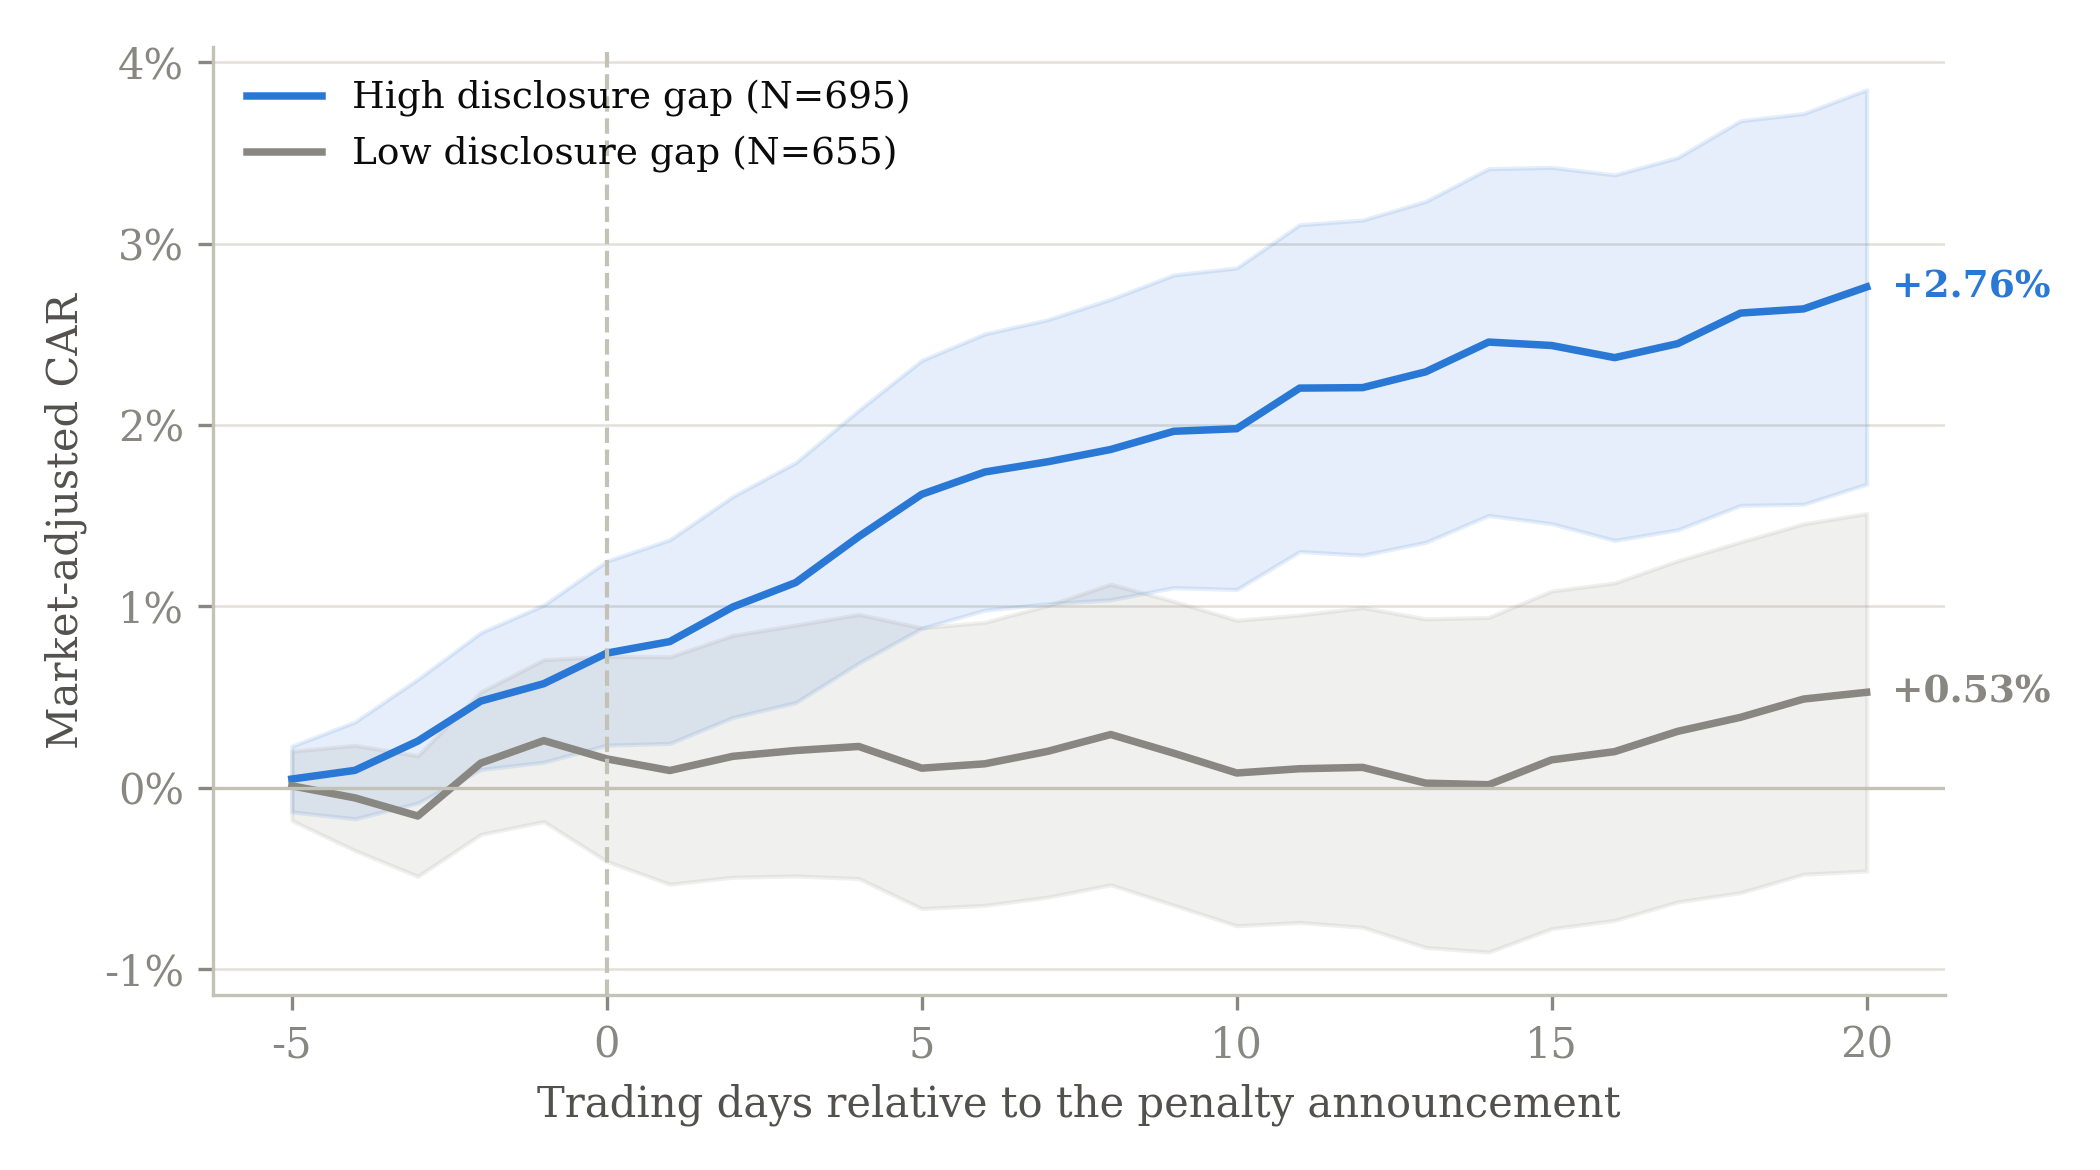
\includegraphics[width=0.82\textwidth]{fig6.png}
\caption{\textbf{Cumulative abnormal returns around penalty announcements.}
Shaded bands are $95\%$ confidence intervals. Baseline timing.}
\label{fig:event}
\end{figure}

\subsection{Not an ESG level, quality, or size effect}
Table~\ref{tab:ic} already shows that ESG performance does not survive style
neutralization. For quality, I build $Q = z(ROA) - z(\textit{Leverage}) -
z(\textit{IdioVol})$; its correlation with \gwsp{} is $0.001$. Adding the
exclusion list on top of a portfolio of the top $30\%$ of $Q$ (dropping 29
stocks per month on average) contributes $0.49\%$ per year with an information
ratio of $0.67$ ($t=2.10$), and in Fama-MacBeth regressions the marginal
$t$-statistic on \gwsp{} is $3.68$ against $0.68$ for $Q$ itself
(Table~\ref{tab:quality}). For size, the double sort in Table~\ref{tab:double}
shows the effect is \emph{stronger} in the large-cap half
(RankIC $=0.0160$, $t=3.63$) than in the small-cap half ($0.0080$, $t=1.57$),
which rules out a micro-cap junk interpretation; the disappearance of the
effect under value weighting (Section~\ref{sec:econ}) is a weighting mechanic,
since excluded names carry very small value weights.

\begin{table}[t]
\centering\small
\caption{\textbf{Marginal contribution on top of a quality composite.}
$Q = z(ROA) - z(\textit{Leverage}) - z(\textit{IdioVol})$; the base portfolio
is the top $30\%$ of $Q$, equal weighted. Excess returns are measured against
the equal-weighted universe.}
\label{tab:quality}
\vspace{6pt}
\begin{tabular}{lccc}
\toprule
& Quality base & Base + exclusion list & Marginal \\
\midrule
Annualized excess & $1.67\%$ & $2.17\%$ & $\mathbf{0.49\%}$ \\
Information ratio & $0.30$ & $0.40$ & $\mathbf{0.67}$ \\
$t$ & $0.93$ & $1.26$ & $\mathbf{2.10}$ \\
\bottomrule
\end{tabular}
\end{table}

%---------------- 6 Mechanism ----------------
\section{Mechanism: liquidity or price discovery?}

\subsection{The liquidity channel is rejected}
Table~\ref{tab:liq} reports three tests of H2 that point the same way. First,
the sign is wrong for the hypothesis: Fama-MacBeth regressions of log
\citet{amihud2002} illiquidity on \gwsp{} give a \emph{positive} coefficient
($0.0407$, $t=15.69$; $0.0414$, $t=16.08$ with size and turnover controls),
meaning relatively silent firms are more liquid. Second, the mediated share is
small: the indirect effect is $7.0\%$ of the total (\citealt{sobel1982} $z=2.34$,
$p=0.019$), and its sign corresponds to the conventional illiquidity premium
rather than to a barrier-induced risk premium. Third, the signal survives:
adding log-Amihud to the neutralization moves the IC only from $0.0136$ to
$0.0128$ ($t=3.90$), and adding price delay as well leaves it unchanged. The
silence discount is therefore not a liquidity premium in disguise.

\begin{table}[t]
\centering\small
\caption{\textbf{The liquidity channel.} Fama-MacBeth cross-sectional
regressions and a three-step mediation test on monthly cross-sections. The
survival rows re-estimate the signal with the indicated variable added to the
monthly orthogonalization.}
\label{tab:liq}
\vspace{6pt}
\begin{tabular}{lcc}
\toprule
Test & Estimate & $t$ / $p$ \\
\midrule
$a$ path: \gwsp{} $\to \ln(\textit{Amihud})$ & $0.0407$ & $t=15.69$ \\
$b$ path: $\ln(\textit{Amihud}) \to$ return (controlling \gwsp{}) & $0.00356$ & $t=2.36$ \\
$c$: total effect & $0.00207$ & $t=3.87$ \\
$c'$: direct effect & $0.00194$ & $t=3.69$ \\
Indirect effect $a\times b$ (mediated share) & $0.000145$ ($\mathbf{7.0\%}$) & $z=2.34$, $p=0.019$ \\
\midrule
IC after adding $\ln(\textit{Amihud})$ to neutralization & $0.0128$ & $t=3.90$ \\
IC after adding $\ln(\textit{Amihud})$ and delay & $0.0128$ & $t=3.91$ \\
\bottomrule
\end{tabular}
\end{table}

\subsection{The price-discovery channel survives}
I measure price delay following \citet{hou2005}: using 52 weeks of weekly
returns, I regress each stock on the contemporaneous market return and then on
the contemporaneous return plus four weekly lags, and define
$\textit{DELAY} = 1 - R^2_{\text{restricted}}/R^2_{\text{unrestricted}}$.
Higher values mean prices absorb market information more slowly. In my sample
the measure averages $0.27$ with a median of $0.19$ and declines monotonically
with size (from $0.304$ in the smallest decile to $0.250$ in the largest), as
in the original study.

Direct evidence is weak: silent firms have marginally higher delay
(Fama-MacBeth coefficient $-0.0016$, $t=-1.71$). The conditional evidence is
strong. Table~\ref{tab:double} and Figure~\ref{fig:double} show the discount is
concentrated where price discovery is slow, and the contrast across delay
groups is larger than across any other environment variable considered.

\begin{table}[t]
\centering\small
\caption{\textbf{Where the silence discount is strongest.} Each panel splits
the sample at the monthly median of the indicated variable. "Tail excess" is
the annualized return of the most silent $10\%$ within the subsample relative
to the subsample mean. Baseline timing.}
\label{tab:double}
\vspace{6pt}
\begin{tabular}{llcccc}
\toprule
Split variable & Subsample & RankIC & $t$ & Tail excess & $t$ \\
\midrule
\multirow{2}{*}{\textbf{Price delay}} & High (barrier high) & $\mathbf{+0.0168}$ & $\mathbf{3.57}$ & $\mathbf{-7.39\%}$ & $\mathbf{-3.54}$ \\
 & Low & $+0.0082$ & $1.66$ & $-3.01\%$ & $-1.57$ \\
\multirow{2}{*}{Idiosyncratic volatility} & High & $+0.0164$ & $3.25$ & $-6.34\%$ & $-2.90$ \\
 & Low & $+0.0103$ & $2.13$ & $-4.66\%$ & $-3.20$ \\
\multirow{2}{*}{Illiquidity} & High & $+0.0089$ & $1.84$ & $-6.38\%$ & $-3.72$ \\
 & Low & $+0.0136$ & $3.24$ & $-3.11\%$ & $-1.78$ \\
\multirow{2}{*}{Market capitalization} & High & $+0.0160$ & $3.63$ & $-5.11\%$ & $-3.18$ \\
 & Low & $+0.0080$ & $1.57$ & $-2.96\%$ & $-1.60$ \\
\bottomrule
\end{tabular}
\end{table}

\begin{figure}[t]
\centering
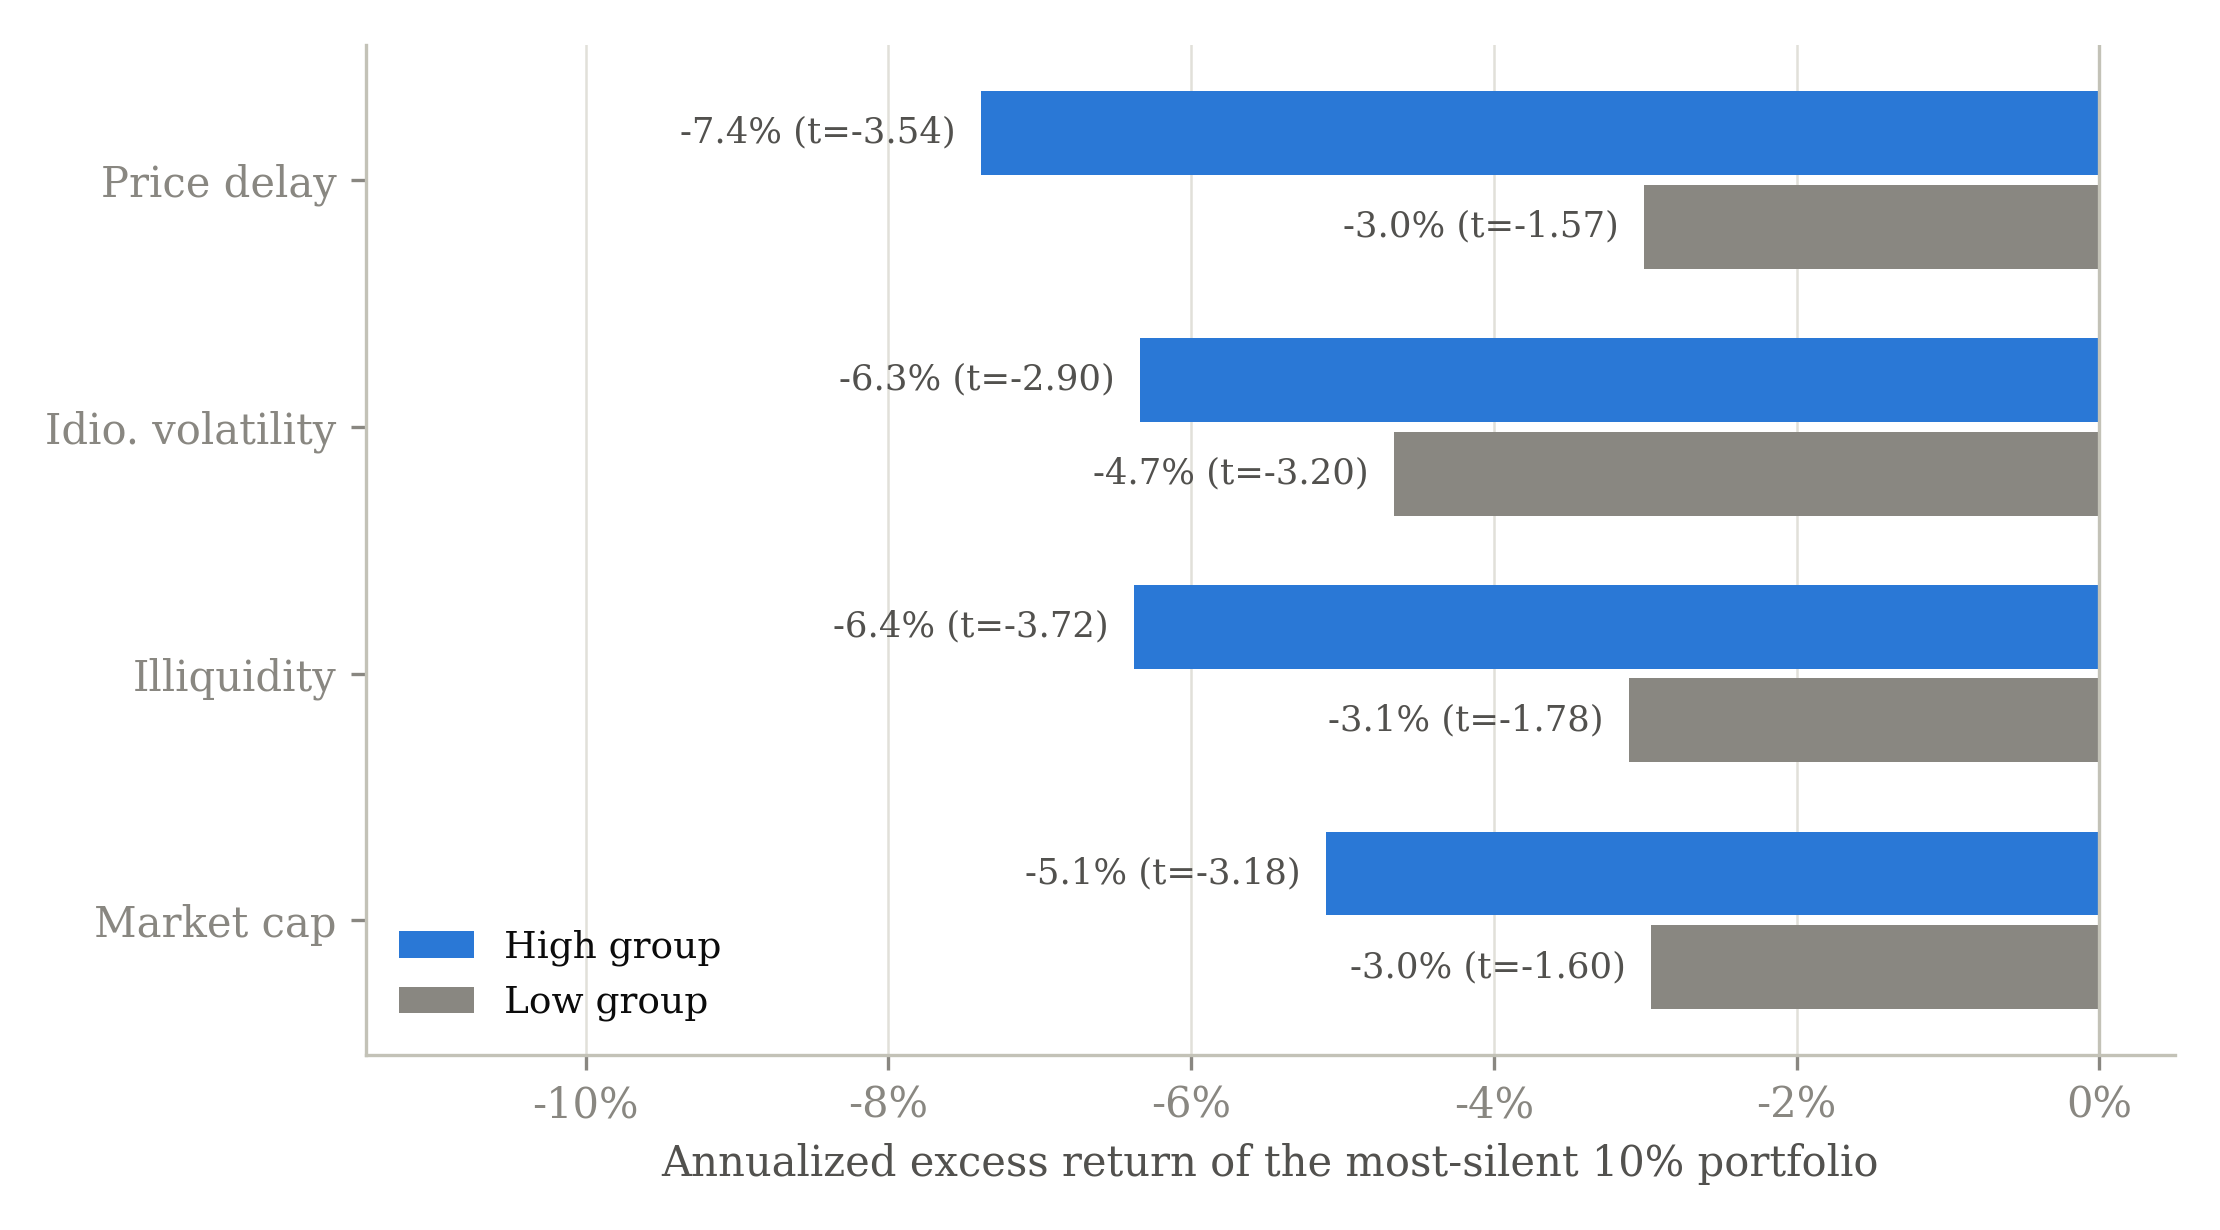
\includegraphics[width=0.86\textwidth]{fig5.png}
\caption{\textbf{Where the silence discount is strongest.} Annualized excess
return of the most-silent decile within each subsample, with $t$-statistics.}
\label{fig:double}
\end{figure}

\subsection{Discriminating price discovery from limits to arbitrage}
Price delay correlates with idiosyncratic volatility ($\rho=0.37$), the
standard proxy for limits to arbitrage, so the previous result could be a
restatement of that friction. Table~\ref{tab:triple} repeats the delay split
\emph{within} the low-volatility half of the sample. Delay continues to
separate the two groups, indicating that price-discovery speed carries
information beyond arbitrage costs.

\begin{table}[t]
\centering\small
\caption{\textbf{Delay split within the low-idiosyncratic-volatility
subsample.} The sample is first restricted to stocks below the monthly median
of idiosyncratic volatility and then split at the median of price delay.}
\label{tab:triple}
\vspace{6pt}
\begin{tabular}{lccccc}
\toprule
Subsample & Stocks/month & RankIC & $t$ & Tail excess & $t$ \\
\midrule
Low volatility $\times$ high delay & 233 & $\mathbf{+0.0160}$ & $\mathbf{2.37}$ & $\mathbf{-5.94\%}$ & $\mathbf{-3.11}$ \\
Low volatility $\times$ low delay  & 233 & $+0.0085$ & $1.34$ & $-3.43\%$ & $-1.93$ \\
\bottomrule
\end{tabular}
\end{table}

Section~\ref{sec:event} completes the picture. Penalty filings act as forced
information releases---moments when the barrier is removed---and firms with the
highest prior gaps earn positive abnormal returns as uncertainty resolves. The
mechanism the evidence supports is therefore: a barrier is raised, prices
adjust more slowly, a discount accumulates, and the discount is repaired when
the barrier falls.

%---------------- 7 Heterogeneity ----------------
\section{Heterogeneity: rating disagreement and index membership}
\label{sec:hetero}

\citet{hu2023} argue that disagreement among raters indicates a murky ESG
information environment. I measure disagreement as the cross-provider standard
deviation of percentile ranks from three providers (5{,}142 firms have at least
two ratings) and split at the monthly median. Table~\ref{tab:disag} shows an
informative asymmetry: ranking information is stronger where disagreement is
low, whereas the tail discount is concentrated where disagreement is high. This
is consistent with the green-fog view---mispricing of the most silent firms is
deepest precisely where professional assessors cannot agree.

An important caveat: the three rating snapshots are current (August 2026),
i.e.\ after the sample period, so this test relies on disagreement being a
persistent firm attribute. I treat it as suggestive rather than conclusive and
have begun archiving monthly snapshots so that the test can be redone with
point-in-time data.

\begin{table}[t]
\centering\small
\caption{\textbf{Rating disagreement and index membership.} Disagreement is
the cross-provider standard deviation of ESG percentile ranks; index membership
uses month-end constituent lists. Tail excess is defined as in
Table~\ref{tab:double}.}
\label{tab:disag}
\vspace{6pt}
\begin{tabular}{llcccccc}
\toprule
Dimension & Subsample & Stocks/month & RankIC & $t$ & Tail excess & $t$ \\
\midrule
\multirow{2}{*}{Rating disagreement} & Low & 445 & $\mathbf{+0.0177}$ & $\mathbf{4.35}$ & $-3.81\%$ & $-1.76$ \\
 & High & 444 & $+0.0088$ & $1.72$ & $\mathbf{-6.34\%}$ & $\mathbf{-3.93}$ \\
\midrule
\multirow{3}{*}{Index membership} & CSI 300 & 191 & $+0.0137$ & $2.26$ & $-2.56\%$ & $-1.14$ \\
 & CSI 500 & 321 & $+0.0137$ & $2.44$ & $-4.83\%$ & $-2.89$ \\
 & Non-index & 384 & $+0.0096$ & $1.69$ & $\mathbf{-6.83\%}$ & $\mathbf{-3.14}$ \\
\bottomrule
\end{tabular}
\end{table}

%---------------- 8 Economic significance ----------------
\section{Economic significance}
\label{sec:econ}

Because the information is concentrated in the lower tail, the natural
implementation is an exclusion flag rather than a linear score: drop the most
silent $10\%$ (89 stocks per month on average) from an equal-weighted
portfolio. Table~\ref{tab:port} reports the results.

Three points deserve emphasis. First, costs are not binding: since the list
covers only a tenth of the portfolio, incremental one-way turnover is $1.06\%$
per month and about nine-tenths of the gain survives 30bp round-trip costs.
Second, a once-a-year list is viable---freezing the list annually
(list turnover $6.3\%$ per month) still yields $0.41\%$ per year ($t=2.43$),
which places almost no demand on execution. Third, capacity is genuinely
limited: under value weighting the excess return disappears, because excluded
names carry small value weights. The economic content of this signal is
confined to equal-weighted or small-cap-tilted mandates.

\begin{table}[t]
\centering\small
\caption{\textbf{Portfolio implementation.} Equal-weighted, monthly rebalanced,
baseline timing. Excess returns are measured against the equal-weighted
coverage universe. Under defensive timing the monthly-refresh variant earns
$0.47\%$ per year with an information ratio of $1.07$ ($t=3.28$).}
\label{tab:port}
\vspace{6pt}
\begin{tabular}{lcccc}
\toprule
& Monthly list & Annual frozen list & After 30bp & Value weighted \\
\midrule
Annualized excess & $0.57\%$ & $0.41\%$ & $0.53\%$ & $-0.19\%$ \\
Tracking error & $0.49\%$ & $0.53\%$ & $0.49\%$ & $1.30\%$ \\
Information ratio & $1.17$ & $0.77$ & $1.09$ & $-0.15$ \\
$t$ & $3.67$ & $2.43$ & $3.44$ & $-0.47$ \\
\% positive months & $67.2$ & $63.0$ & $66.4$ & $51.3$ \\
Profit factor & $2.43$ & $1.82$ & --- & --- \\
Max relative drawdown & $-0.44\%$ & $-0.68\%$ & --- & --- \\
List turnover (monthly) & $17.9\%$ & $6.3\%$ & --- & --- \\
Incremental one-way turnover & $1.06\%$ & n.a. & $1.06\%$ & --- \\
\bottomrule
\end{tabular}
\end{table}

%---------------- 9 Robustness ----------------
\section{Robustness and a failed identification attempt}
\label{sec:robust}

\noindent\textbf{Timing.} Moving the application date from January to July of
$t+1$ lowers the RankIC from $0.0124$ ($t=3.45$) to $0.0103$ ($t=2.87$) and the
portfolio gain from $0.57\%$ to $0.47\%$---an attenuation of roughly $15\%$
with no change in conclusions.

\noindent\textbf{Standardization.} Replacing industry standardization with
industry-by-year standardization, which removes any cross-year reuse of
standardization constants, leaves the results unchanged (it is part of the
defensive specification).

\noindent\textbf{Signal age.} Splitting months by how long the annual signal
has been in use, the RankIC is $0.0123$ ($t=2.30$) in the first six months and
$0.0125$ ($t=2.58$) in the last six. The signal captures a slow-moving firm
attribute rather than news, and annual updating costs nothing.

\noindent\textbf{Alternative construction.} A signal built directly from the
residualized disclosure score, without forming a gap at all, correlates $0.971$
with \gwsp{} and performs almost identically (IC $=0.0142$, $t=4.21$). After
full neutralization the "disclosure minus performance" gap is effectively a
measure of \emph{conditional disclosure}; the performance leg mainly serves an
orthogonalizing role.

\noindent\textbf{Real outcomes.} In the annual firm panel with industry and
year fixed effects and clustered standard errors, the disclosure gap enters ROA
with a coefficient of $0.0111$ ($t=3.73$) once ESG performance is controlled
(and $-0.0042$, $t=-2.23$, without it---a textbook suppression pattern), and
the result is unchanged using one-year-ahead ROA or $1\%/99\%$ winsorization.

\noindent\textbf{A failed identification attempt.} I attempted to use the April
2024 sustainability-reporting guidelines as an exogenous removal of the
information barrier in a difference-in-differences design, and abandoned the
test for three reasons. First, China's revised "Nine Guidelines" for capital
market development were released on \emph{the same day} (12 April 2024) and
triggered a sharp large-cap/small-cap divergence; my treatment proxy is built
from market capitalization and therefore overlaps the beneficiaries of that
shock, so the two cannot be separated. Second, the event window coincides with
a period in which the baseline effect had itself reversed sign, leaving no
discount whose narrowing could be detected. Third, the triple-difference
estimate is insignificant ($2.2\%$ annualized, $t=0.21$) and size-stratified
estimates swing between $-49\%$ and $+38\%$. I report this as a negative result
rather than dropping it; the natural replacement is to wait until mandatory
reports for fiscal 2025 are filed and use \emph{observed changes in disclosure}
instead of membership proxies.

%---------------- 10 Conclusion ----------------
\section{Conclusion}

Among Chinese listed firms that look alike in size, style, industry, and
realized ESG performance, those that disclose relatively little earn lower
subsequent returns---about $4.2\%$ per year for the bottom decile relative to
comparable firms, robust to the CAPM, Fama-French, and China three-factor
adjustments. The effect is not the mirror image of greenwashing punishment: a
governance placebo is equally strong, polluting industries show no
amplification, and penalty announcements produce positive abnormal returns. It
is not a liquidity premium: silent firms are more liquid and the mediated share
is $7\%$. The channel that survives is price discovery---the discount
concentrates where prices adjust slowly, and this is not merely a limits-to-
arbitrage effect.

Three limitations bound these conclusions. This is a predictability study, not
a causal one: disclosure is chosen, and neutralization controls observables
only. The magnitudes are modest---a monthly IC around $0.012$ and a portfolio
gain around half a percent per year---so the natural use of the signal is as a
low-correlation component or exclusion list within a broader model, not as a
standalone strategy. And coverage is limited to the roughly $970$ Bloomberg-rated
firms per month, about a fifth of the market and tilted large, so extrapolation
to uncovered firms is unwarranted. A twelve-month rolling RankIC turned
negative after the second half of 2023 and the long-short portfolio lost
$1.7\%$ in 2024, plausibly as tightening disclosure rules compressed the very
dispersion this paper exploits; a twenty-four-month window has not yet turned,
so the sample cannot yet say whether the effect has decayed permanently.

Three extensions follow directly. Broader ESG coverage would allow the
extensive margin---firms that disclose nothing at all---to be studied, which is
the most extreme form of the silence documented here. Once fiscal-2025
mandatory reports are filed, observed disclosure changes offer a cleaner
identification strategy than the one that failed here. And textual measures of
disclosure specificity and promise fulfillment would separate "silence" from
"empty talk," a distinction this paper's score-based measure cannot make.

\newpage
\bibliographystyle{plainnat}
\bibliography{references}

\end{document}
